\documentclass[a4paper,10pt]{jsarticle}

% レイアウト
\setlength{\textwidth}{\fullwidth}
\setlength{\textheight}{39\baselineskip}
\addtolength{\textheight}{\topskip}
\setlength{\voffset}{-0.5in}
\setlength{\headsep}{0.3in}
\pagestyle{myheadings}

% パッケージ
\usepackage[dvipdfmx]{graphicx}
\usepackage{amsmath,amssymb,epsfig}
\usepackage{bm}
\usepackage{ascmac}
\usepackage{pifont}
\usepackage{multirow}
\usepackage{enumerate}
\usepackage{cases}
\usepackage{type1cm}
\usepackage{cancel}
\usepackage{url}
\usepackage[dvipdfmx]{color}
\usepackage{listings,jlisting}
% 大きな中括弧
\usepackage{cases}

% 定義
\DeclareMathOperator*{\argmin}{arg\,min}
\DeclareMathOperator*{\argmax}{arg\,max}
\def\vec#1{\mbox{\boldmath$#1$}}
\def\R{{\Bbb R}}

% カウンタの設定
\setcounter{section}{0}
\setcounter{subsection}{0}
\setcounter{subsubsection}{0}
\setcounter{equation}{0}

% キャプションの図をFigに変更
\renewcommand{\figurename}{Fig.}
\renewcommand{\tablename}{Tab.}

% 式番号を式(章番号.番号)に
% \makeatletter
% \renewcommand{\theequation}{\arabic{section}.\arabic{equation}}
% \@addtoreset{equation}{section}
% \makeatother

% プログラムに色をつける
\usepackage{color}

\definecolor{codegreen}{rgb}{0,0.6,0}
\definecolor{codegray}{rgb}{0.5,0.5,0.5}
\definecolor{codepurple}{rgb}{0.58,0,0.82}
\definecolor{backcolour}{rgb}{0.95,0.95,0.92}

\lstdefinestyle{mystyle}{
    backgroundcolor=\color{backcolour},
    commentstyle=\color{codegreen},
    keywordstyle=\color{magenta},
    numberstyle=\tiny\color{codegray},
    stringstyle=\color{codepurple},
    basicstyle=\footnotesize,
    breakatwhitespace=false,
    breaklines=true,
    captionpos=b,
    keepspaces=true,
    numbers=left,
    numbersep=5pt,
    showspaces=false,
    showstringspaces=false,
    showtabs=false,
    tabsize=2
}

\lstset{style=mystyle}

% % ドキュメントの開始
\begin{document}

\section{実行方法}
\subsection{動作環境}
LinuxのディストリビューションのひとつであるUbuntuで動作を確認している.
Ubuntuで動作させるための必要なアプリケーションは以下の通りである.

\begin{lstlisting}[basicstyle=\ttfamily\footnotesize, language=Bash, frame=single, firstnumber=1, numbers=left, breaklines=true]
sudo apt-get install build-essential
sudo apt-get install cmake
sudo apt-get install gnuplot
\end{lstlisting}

コンパイル時に必要なビルドシステムはbuild-essentialとcmakeが必要であり,可視化のためにgnuplotを用いている.

\subsection{コンパイル方法と実行方法}

\begin{lstlisting}[basicstyle=\ttfamily\footnotesize, language=Bash, frame=single, firstnumber=1, numbers=left, breaklines=true]
mkdir build
cd build
cmake ..
make
./実行ファイル名
\end{lstlisting}

\section{課題内容}
\subsection{課題1}
\subsubsection{(a)}
$X_0$軸周り,$Y0$軸周り,$Z0$軸周り,の順番に回転する計算方法は以下の通りであり,処理結果の図形をFig.~\ref{fig:課題1(a)}に示す.


\begin{figure}[htb]
  \begin{center}
    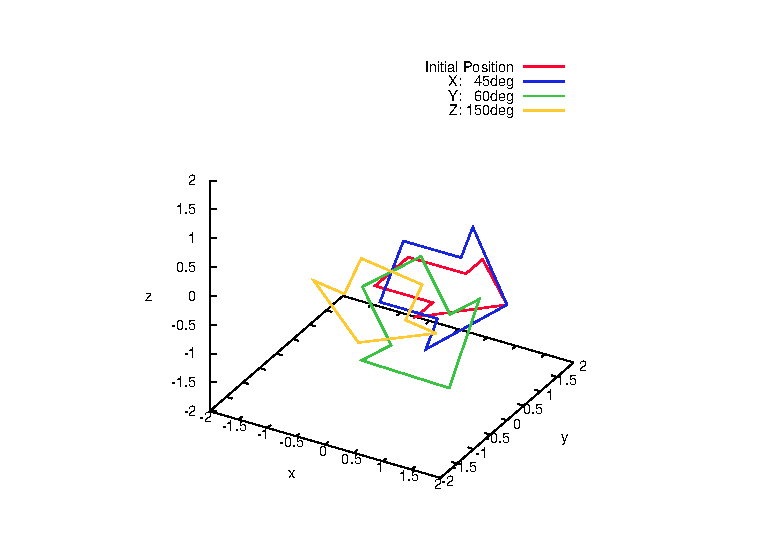
\includegraphics[clip,width=14cm]{fig/eps/1(a).eps}
  \end{center}
  \caption{課題1(a)}
  \label{fig:課題1(a)}
\end{figure}

\begin{figure}[htb]
  \begin{center}
    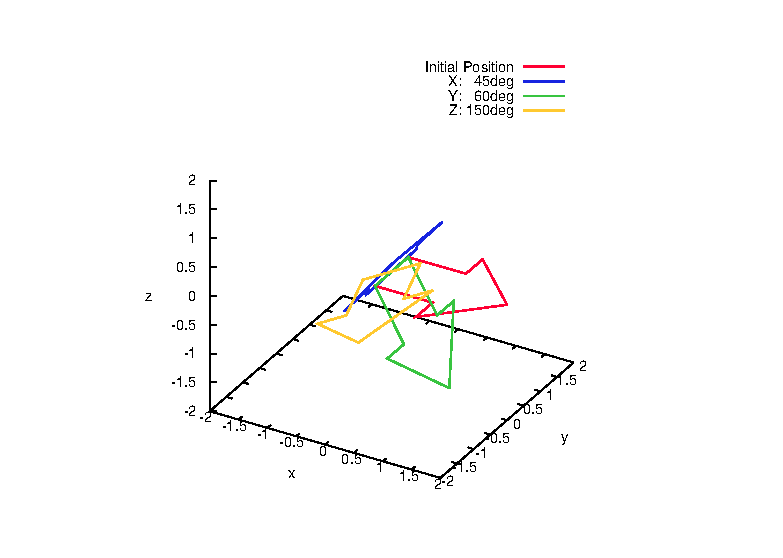
\includegraphics[clip,width=14cm]{fig/eps/1(b).eps}
  \end{center}
  \caption{課題1(b)}
  \label{fig:課題1(b)}
\end{figure}

\begin{figure}[htb]
  \begin{center}
    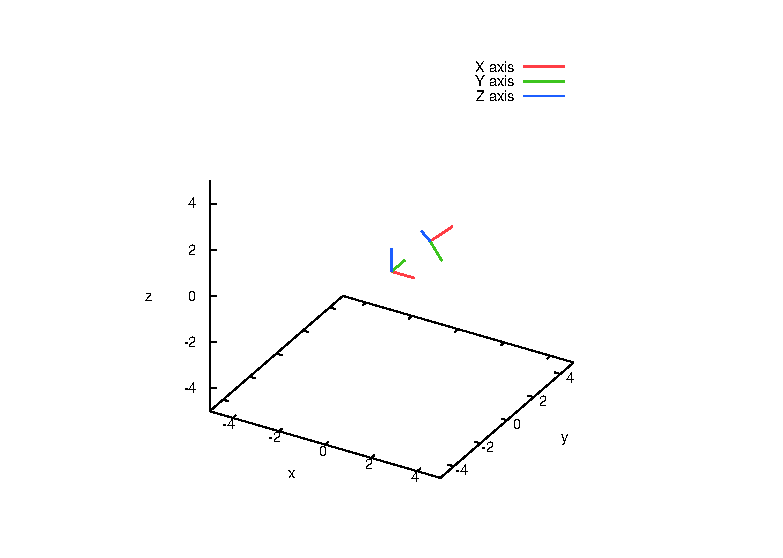
\includegraphics[clip,width=14cm]{fig/eps/2.eps}
  \end{center}
  \caption{課題2}
  \label{fig:課題2}
\end{figure}

\begin{figure}[htb]
  \begin{center}
    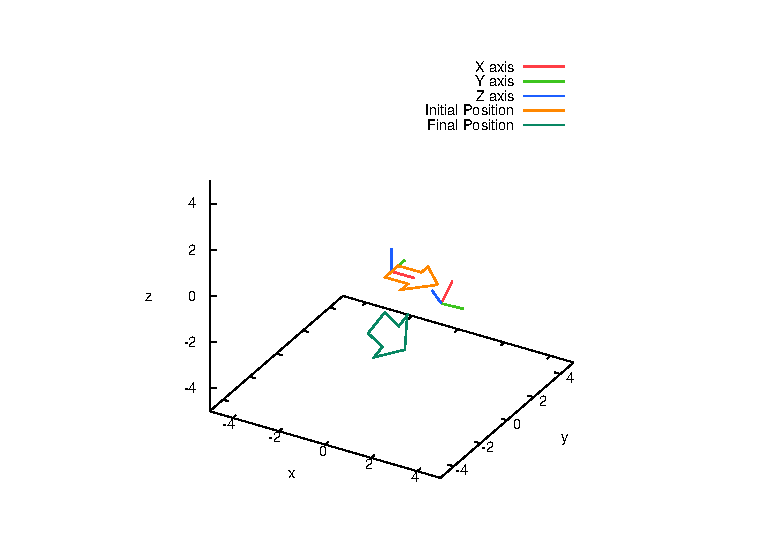
\includegraphics[clip,width=14cm]{fig/eps/3.eps}
  \end{center}
  \caption{課題3}
  \label{fig:課題3}
\end{figure}

\begin{figure}[htb]
  \begin{center}
    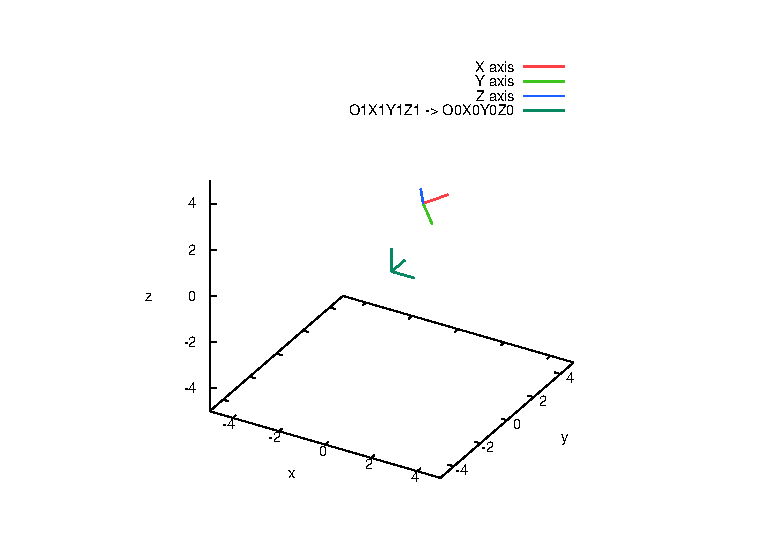
\includegraphics[clip,width=14cm]{fig/eps/4.eps}
  \end{center}
  \caption{課題4}
  \label{fig:課題4}
\end{figure}

\begin{figure}[htb]
  \begin{center}
    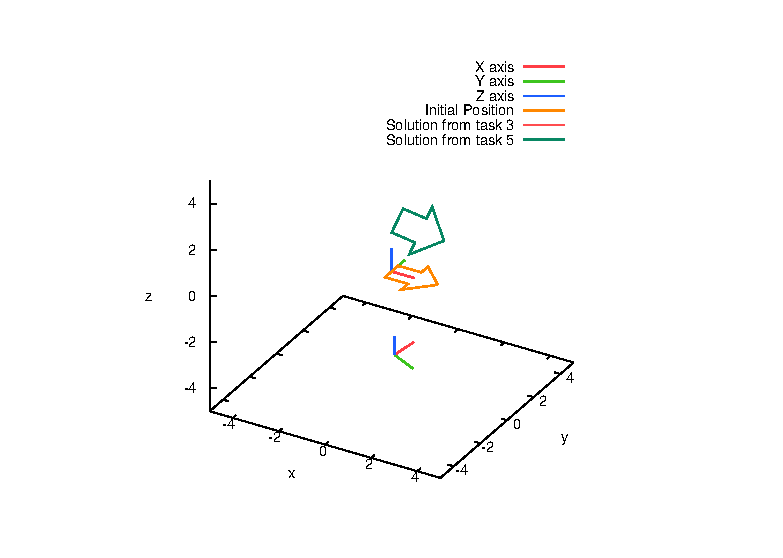
\includegraphics[clip,width=14cm]{fig/eps/5.eps}
  \end{center}
  \caption{課題5}
  \label{fig:課題5}
\end{figure}

\end{document}